\chapter{Implementation} \label{Chapter:Implementation}
intro here

\section{Finding genre combinations}

Today's most popular game store on PC, Steam \cite{steam}, which, at the time of writing, has a library of over 204.000 apps, including the majority of modern video games. There are some exceptions, however, as some games are platform-specific and thus have never been released on Steam, but the quantity of such games can only be measured in the hundreds, so they will be considered insignificant for this research.

To categorize this massive amount of content, Steam uses two systems. First, developers and publishers pick from a list of pre-defined genres to assign to their apps during upload. Second, users who download these apps can assign them user-defined tags that can indicate genre, theme, aesthetic or even difficulty, and help other users find new apps that are to their liking. From the user's point of view, only the tags are visible on the apps' dedicated pages while genres are only used as filtering in the store's search field.

Steam has a public API (Application Programming Interface) that can be used to query data about their games and apps. This API, however, is not well-documented, thus it would take a considerable amount of trial-and-error to use it properly. Luckily, a relatively fresh dataset \cite{steamCatalogInsight2024} can be found on GitHub that, according to the author, was acquired in October 2024 using the Steam API and contains all the data necessary to find existing genre combinations on Steam. To check exactly how up-to-date this data set is, I checked the number of games under some tags on Steam and compared them to the numbers found in the data set, and the differences were around 40\%, which is unexpectedly high. However, games released in October 2024 can be found in the data set as expected with the correct release dates, indicating the data was truly acquired in or after October 2024. The explanation for such a large difference in the numbers could be explained by the ever-rising number of new games published each month on the platform, and the new tags applied to games during this two-month period. However, the ratio between the tag occurrences could not change significantly under such a short time. These data are in CSV format which is mostly used by spreadsheet editors such as Excel or Numbers, but can easily be read from script too.

Going through the data set and individually counting the times each tag occurs, it is easy to determine that Steam currently uses 447 tags and 121 genres. It can also be observed that tag occurrences, as seen in the figure \ref{figure:tags}, like many other data sets, seem to loosely follow Zipf's law \cite{li2002zipf}. Interestingly, some of the tags make little sense, like "Intentionally Awkward Controls" or "TrackIR", and do not represent a genre, but rather some other aspect of the game. There are a few tags like "Warhammer 40K" that solely indicate which franchise the game belongs to.

\begin{figure}[h]
    \centering
    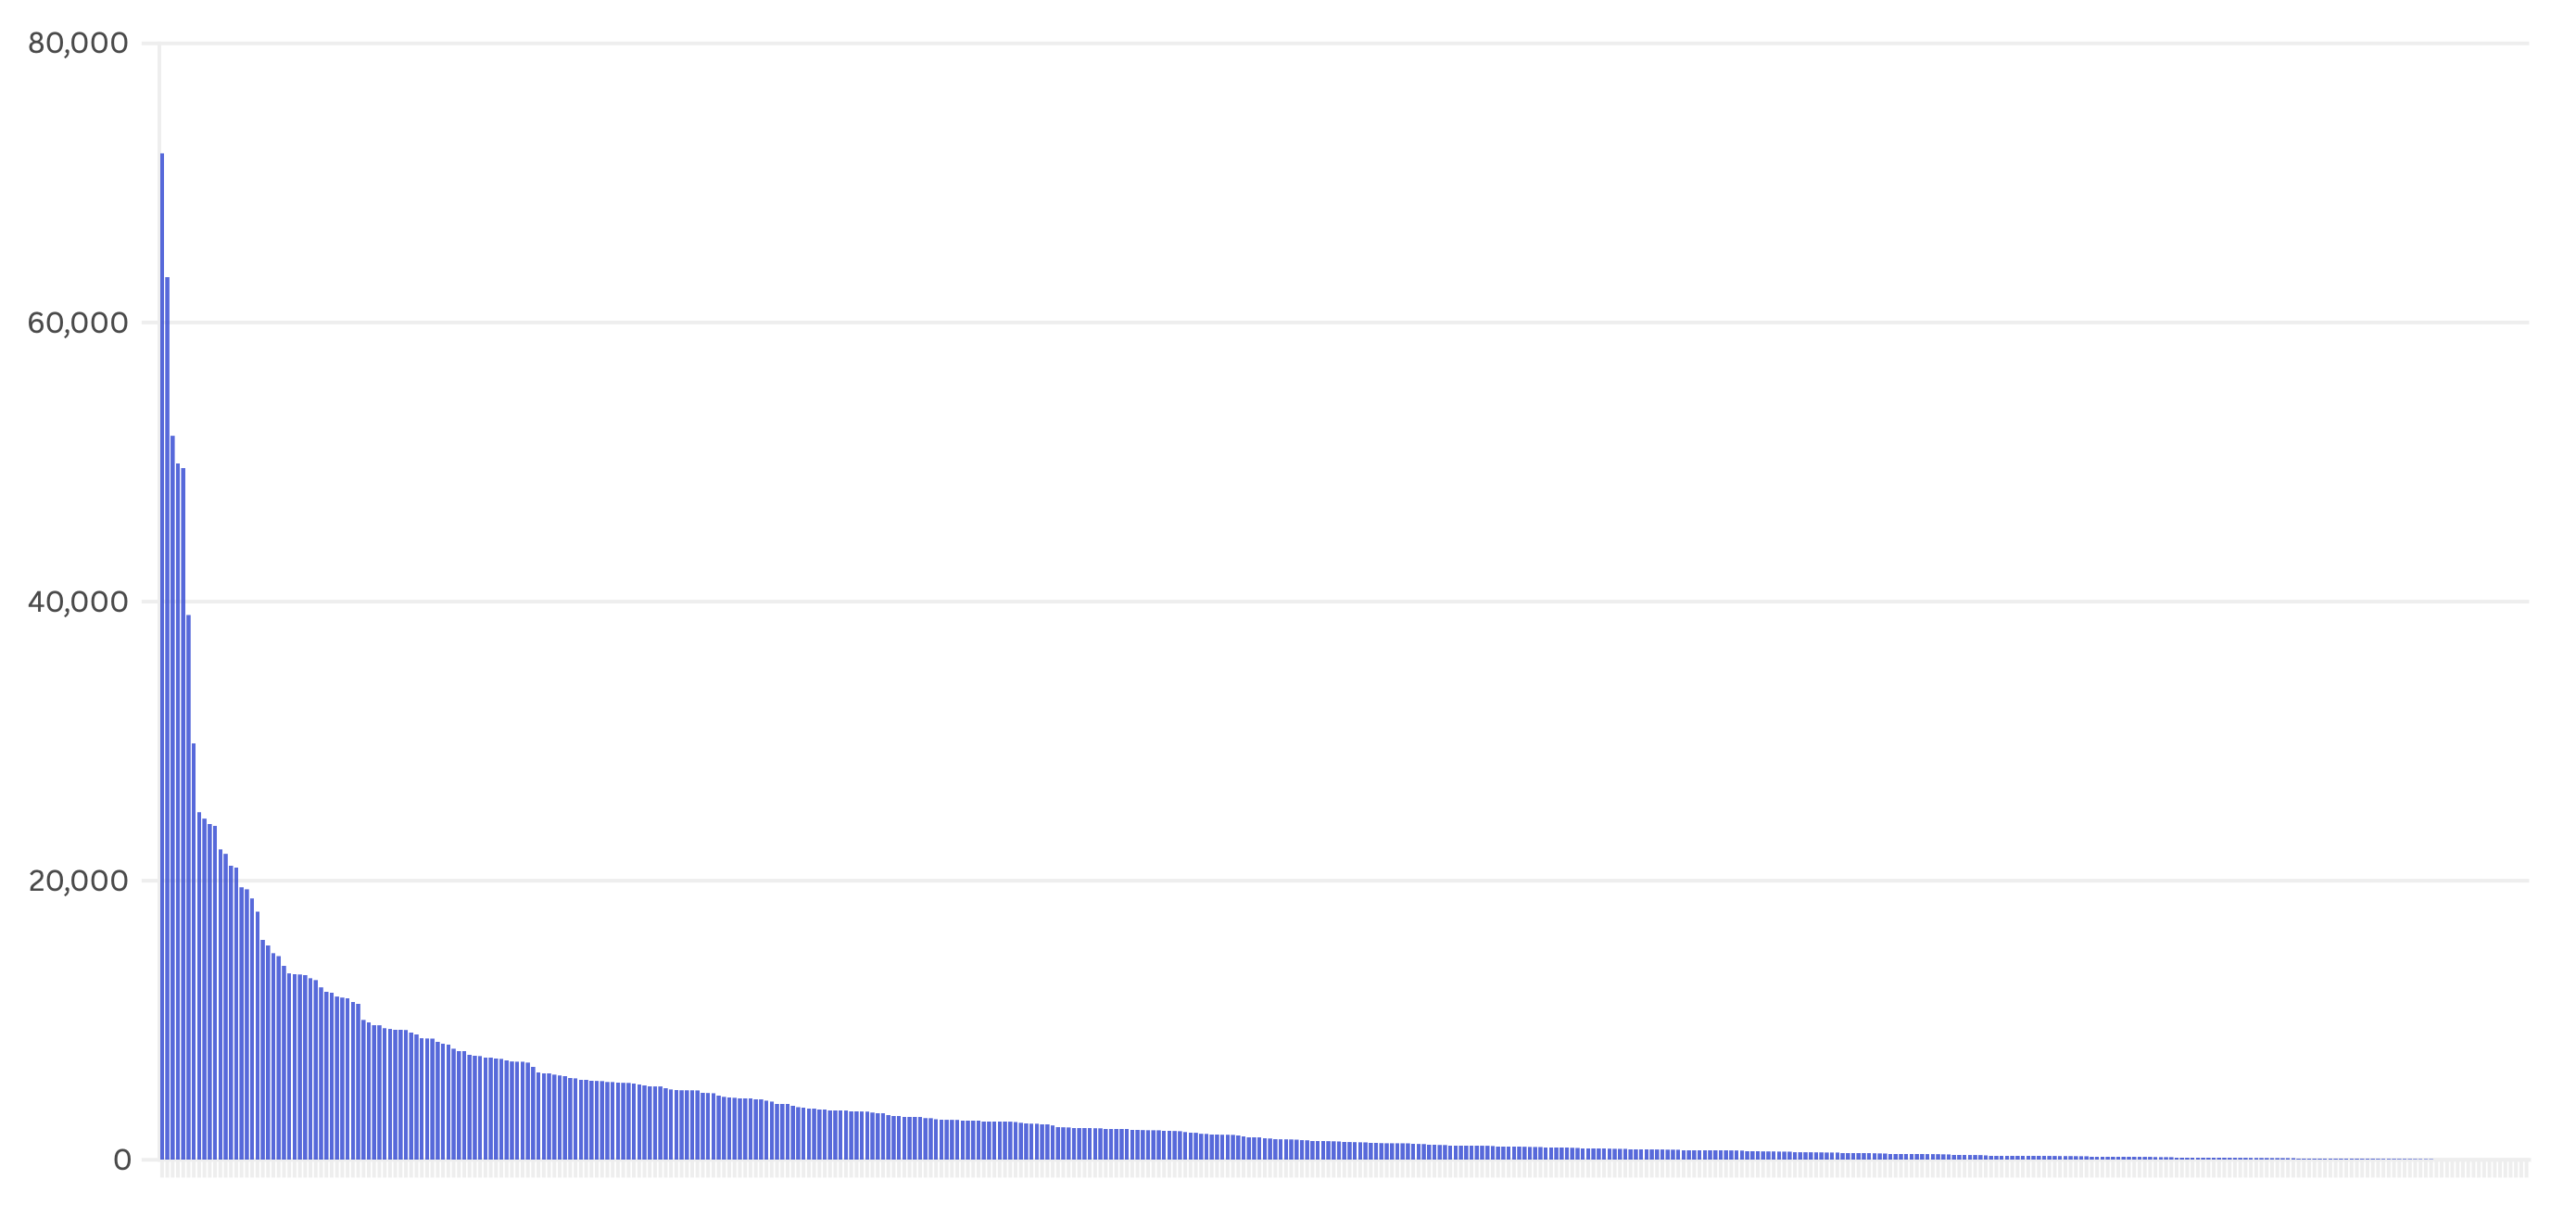
\includegraphics[width=\textwidth]{images/tag-occurrences.png}
    \caption{Tag occurrences}
    \label{figure:tags}
\end{figure}

On the other hand, the genre distribution in the figure \ref{figure:genres} seems unbalanced. The reason for that is that for some reason, 84 of the 121 genres are localized versions of others, and each appear less than 30 times. These genres can be safely discarded, as their occurrance times would not contribute too much to the other numbers.

However, since Steam uses only a handful of genres to categorize games, these genres are vague. For this thesis, I will use Steam tags, as tags provide a much finer way to describe what genres the developed game prototype should belong to.

\begin{figure}[h]
    \centering
    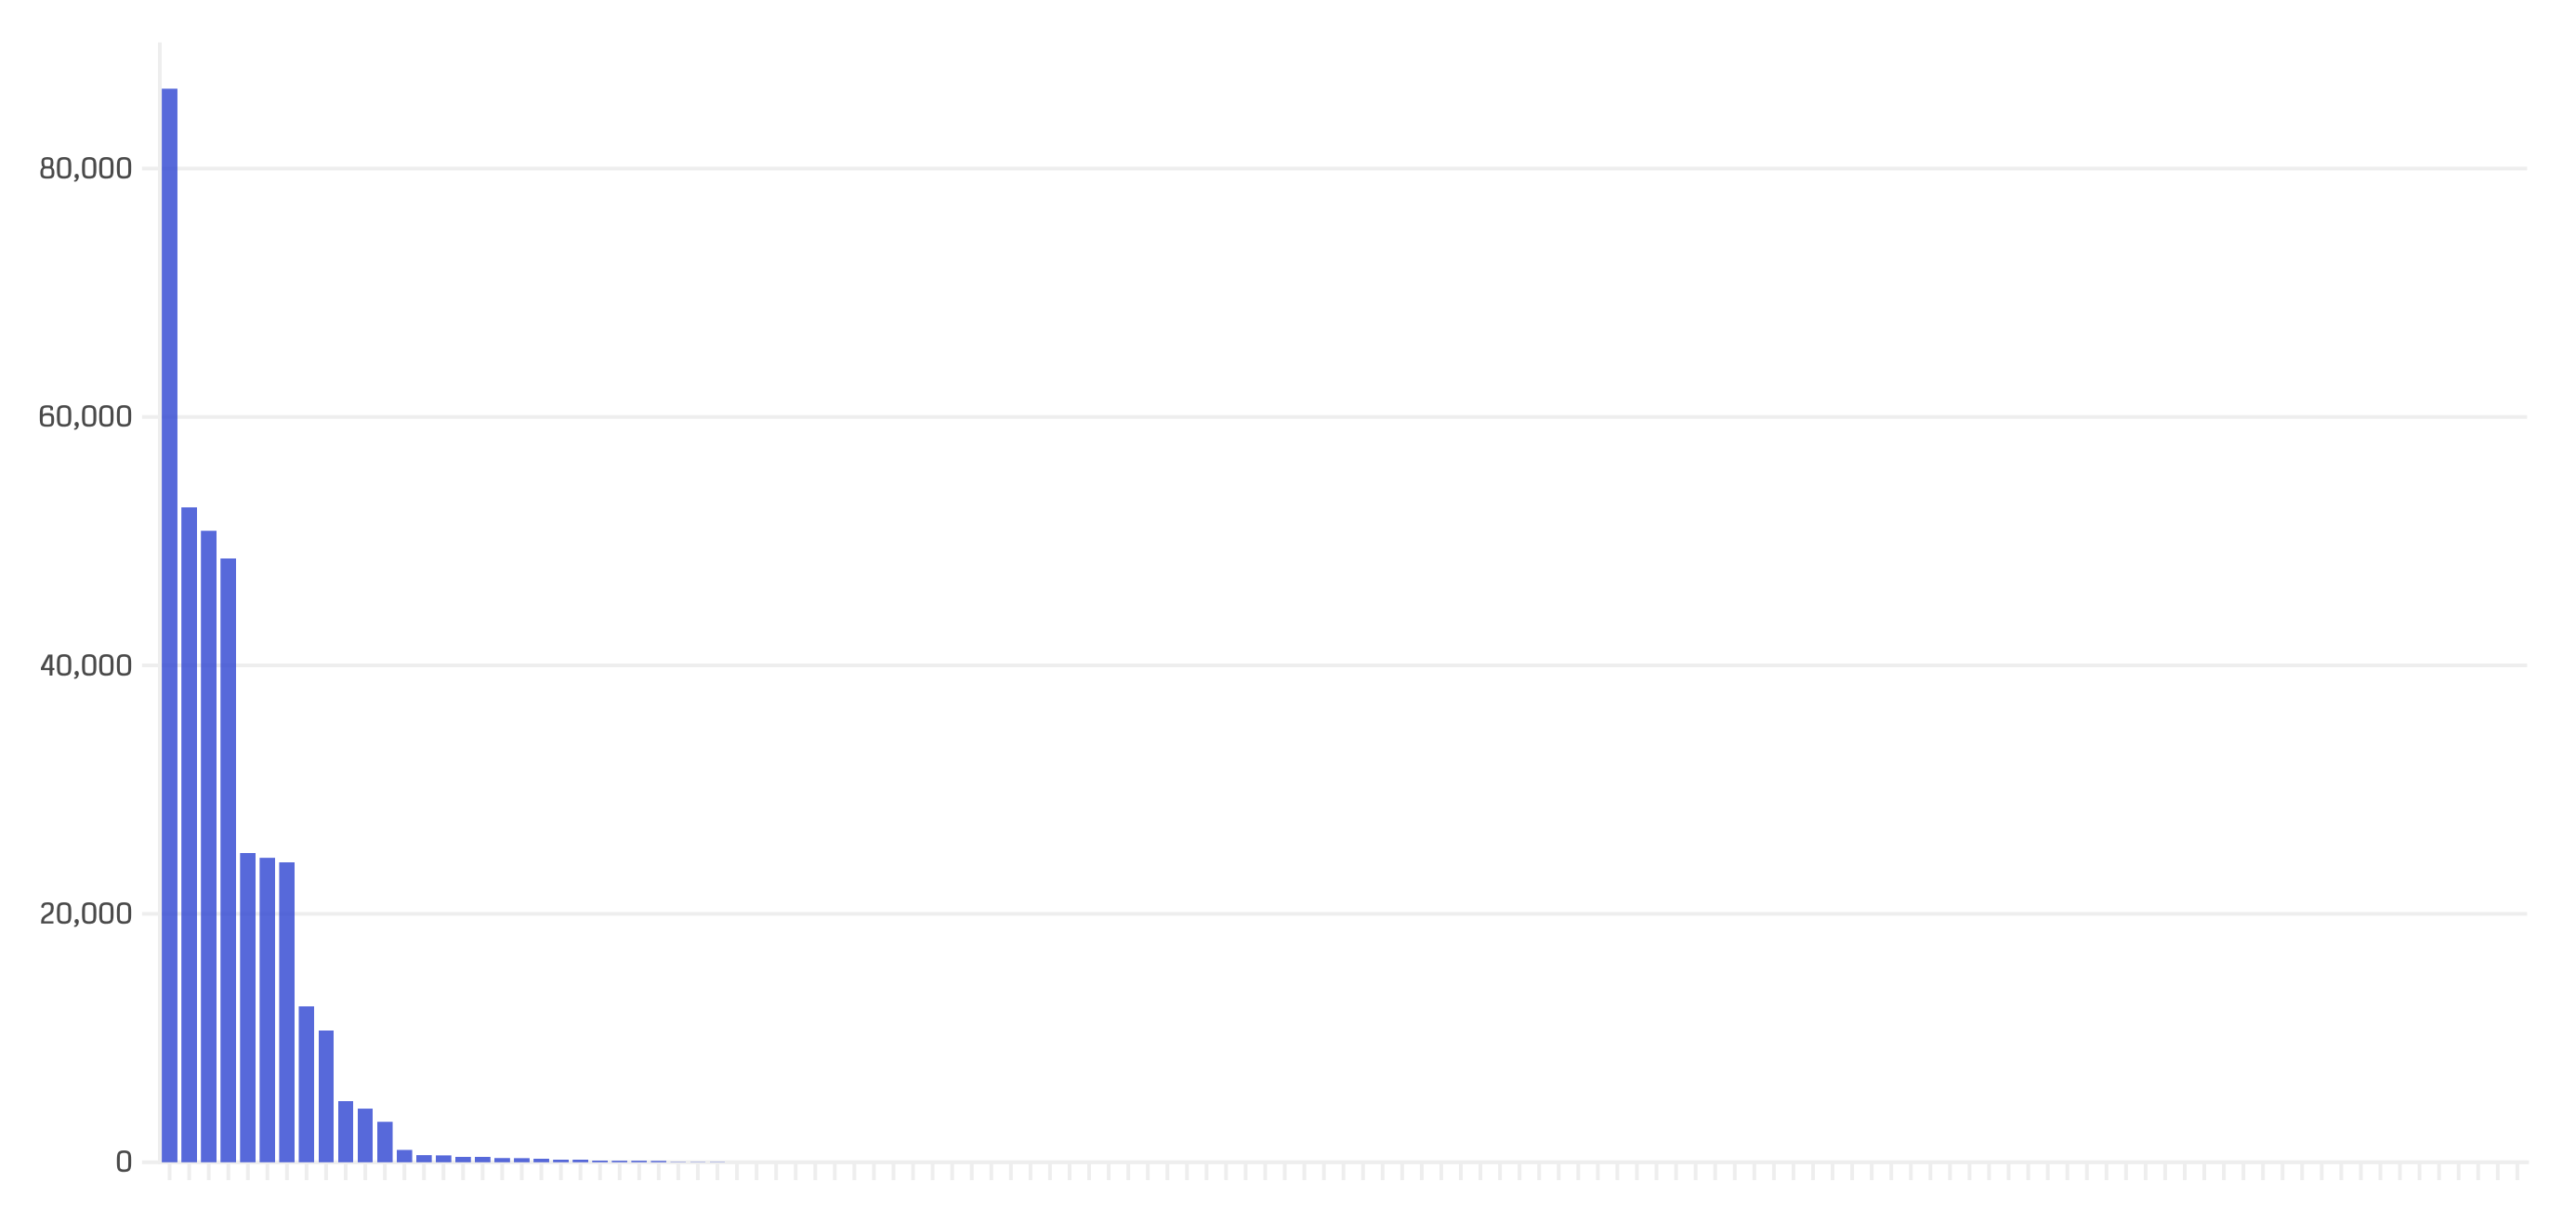
\includegraphics[width=\textwidth]{images/genre-occurrences.png}
    \caption{Genre occurrences}
    \label{figure:genres}
\end{figure}

It is important to note that the author of the dataset also looked for genre combinations as seen in figure \ref{figure:genre-pairs}, but they only used combinations of two genres, while I was more interested in more complex mixtures. Furthermore, they only included tags were assigned to at least 900 games, and takes away almost half of the tags. For this thesis, I am interested in the other half of the tags, those that are used very rarely, but at the same time, clearly represent a genre or sub-genre. To extract exactly the data I needed, I had to write my own script.

\begin{figure}[h]
    \centering
    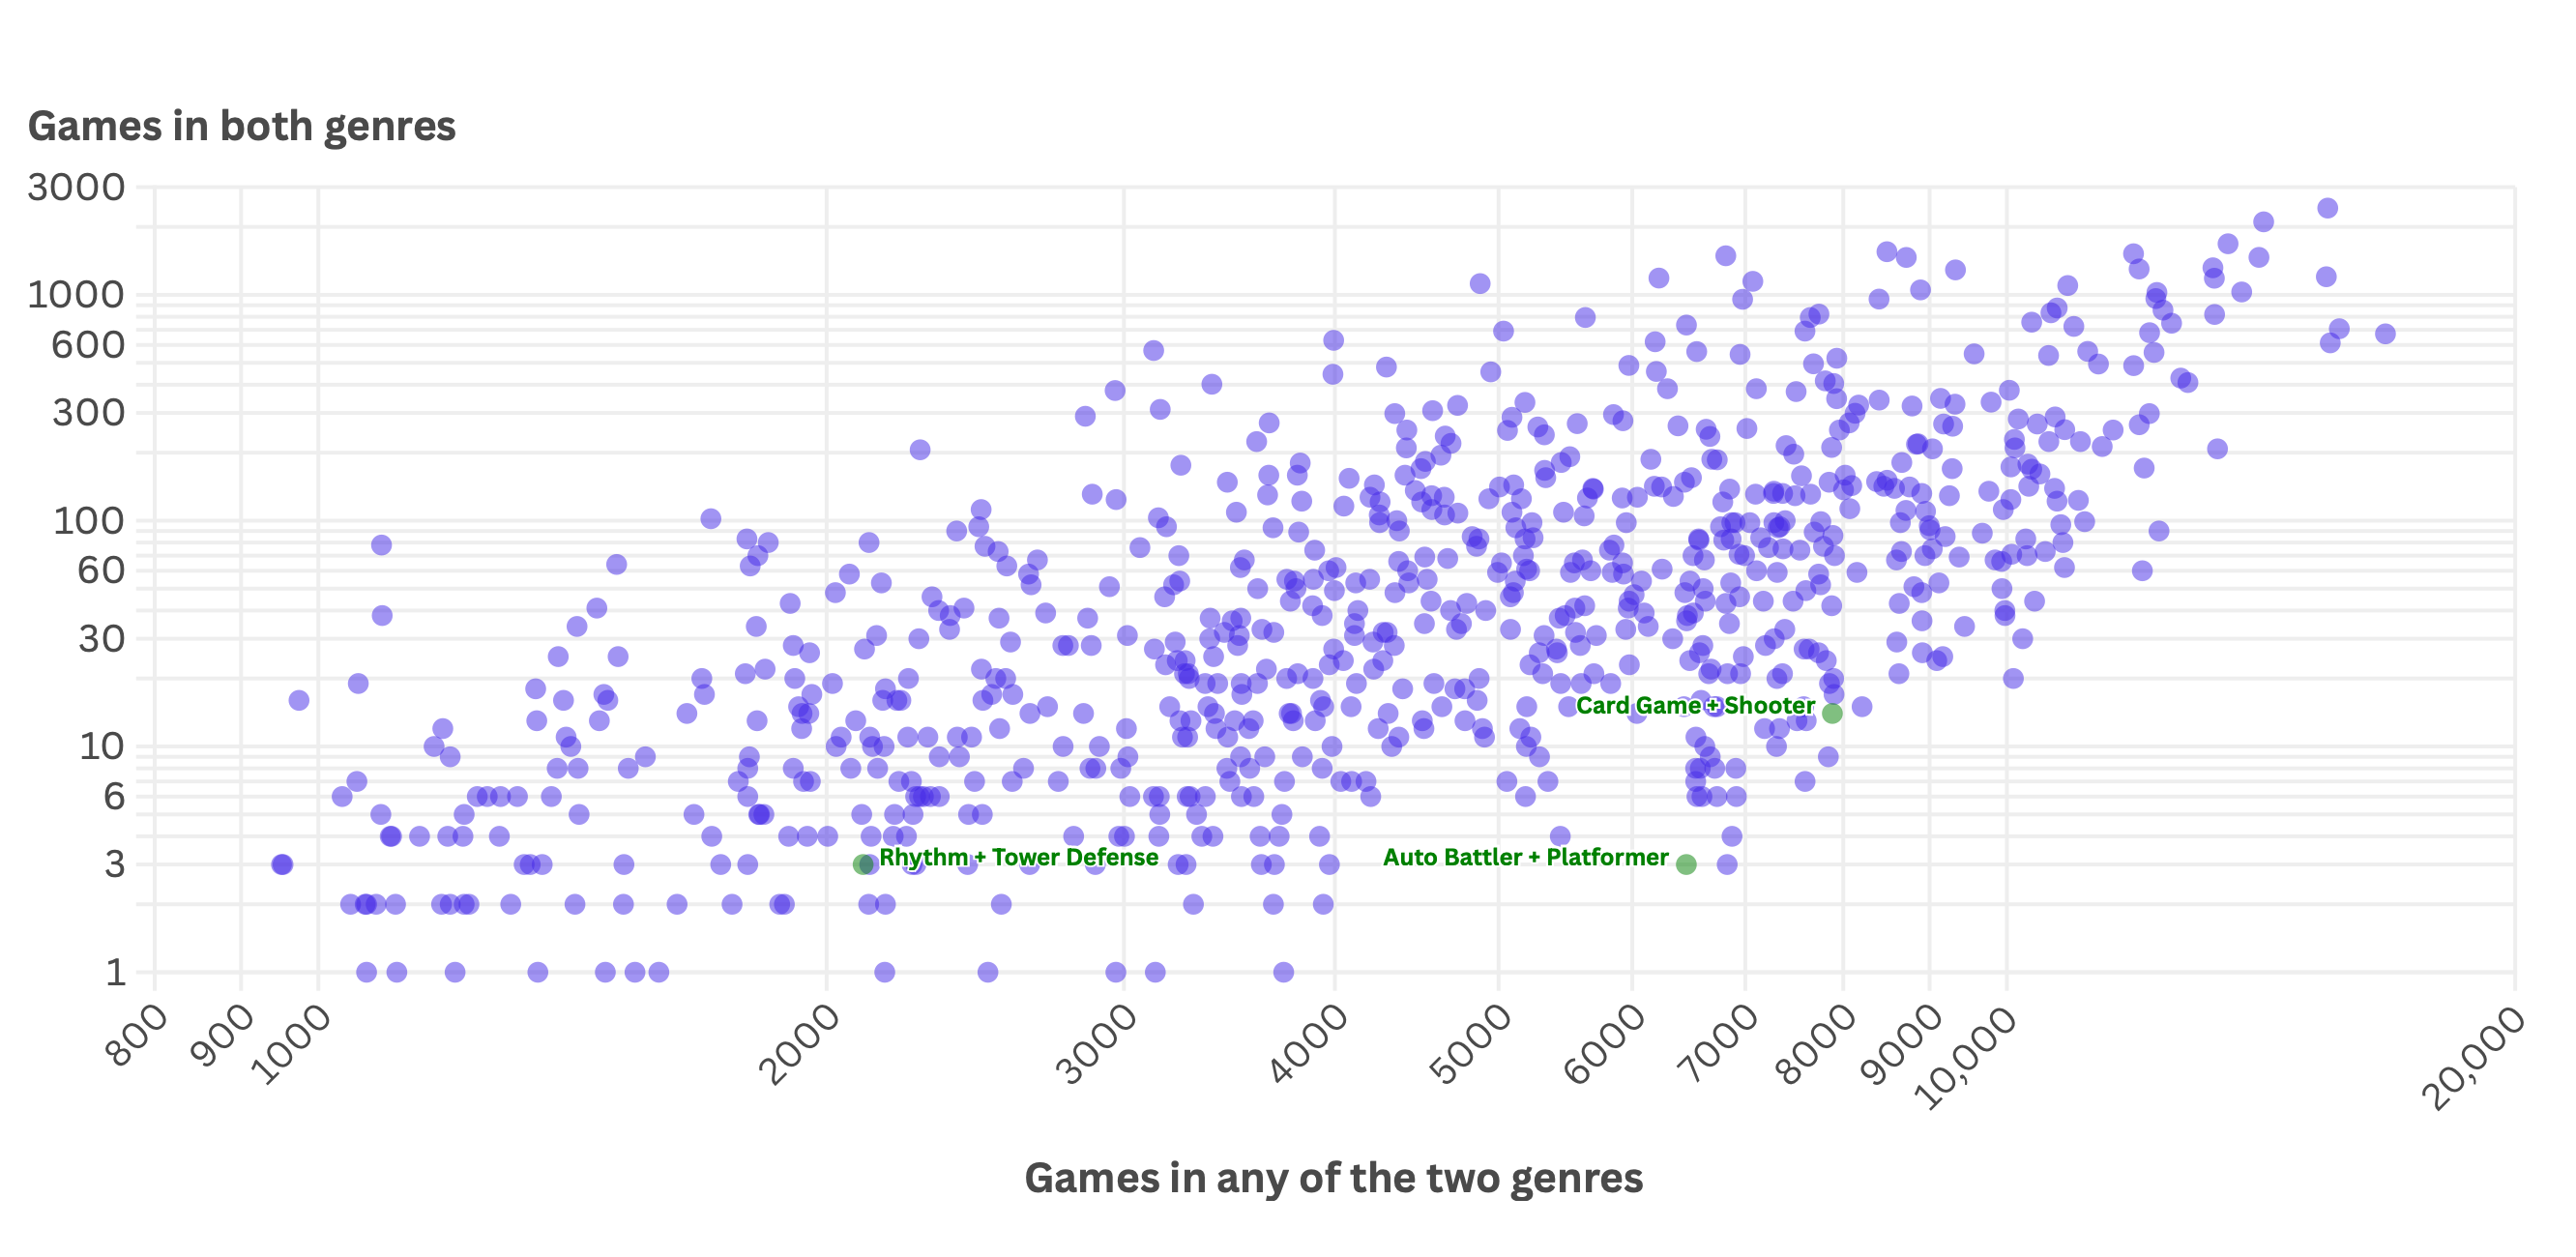
\includegraphics[width=\textwidth]{images/genre-pairs.png}
    \caption{Most frequent genre pairs}
    \label{figure:genre-pairs}
\end{figure}

\section{Research question 1}

After reviewing the data set and going through the less-popular tags, filtering out those that do not represent a genre or sub-genre.

